\documentclass{article}

% --- load packages ---

\usepackage[margin=1in]{geometry} % change the margins
\usepackage{amsmath} % useful math environments and commands like align
\usepackage[colorlinks,bookmarks,bookmarksnumbered,allcolors=blue]{hyperref} % hyperlinks between references
\usepackage{graphicx}  % include images
\usepackage[caption=false]{subfig} % subfigures.  false option prevents conflicts in caption styling with other packages
\usepackage{booktabs} % better tables
\usepackage[capitalise]{cleveref} % better referencing. uses cref.
\usepackage[section]{placeins} % sometimes useful to prevent figures from floating out of a section
\usepackage{cite} % handles multiple citations in one command better
\usepackage{doi} % allow correct hypderlinking of DOIs
\usepackage{hyperref}


\begin{document}

\title{Homework 2}
\author{Jaron Ellingson\\
Pseudoname: jdawg}
% put in \date{} if you don't want a date to appear, or enter a specific date, otherwise default is today's date.
\maketitle

 %\href{https://byu.box.com/shared/static/anxheci3eytucrh3ke57k2sqdx0ivmjg.pdf}{homework pdf}

\section*{Algorithms}

The following describes and compares several unconstrained optimization techniques which all rely on analytical gradients. These algorithms are based on this hyperlinked \href{https://byu.box.com/shared/static/17bqmaop0v1o0fwqg1etx7dofl6ad35t.pdf}{textbook} that provides an in depth description in chapter 3. I chose to implement two line-search algorithms (section 3.4 in the textbook), simple backtracking and the algorithm presented in \cite{nocedal2006numerical}, which I will refer to as the N-W algorithm. Additionally, I implemented two search direction algorithms (section 3.5 in the textbook), steepest descent and Quasi-Newton algorithms. These algorithms each have their pros and cons and I will briefly describe each of them.

\subsection*{Line Search}

Both of the line search algorithms take advantage of the fact that the current line search is roughly the same as the next line search. This means that, 

\begin{equation*}
\begin{aligned}
\alpha_k g_k^T p_k  & \approx \alpha_{k-1} g_{k-1}^T p_{k-1} \\
\alpha_k & \approx \alpha_{k-1} \frac{||g_{k-1}||^2}{||g_{k}||^2}, \\
\end{aligned}
\end{equation*}

where $\alpha_k$ is out current step size, $g_k$ is our gradient, and $p_k$ is our search direction.

\subsubsection*{Backtracking}

The backtracking algorithm relies on the fact that our search direction is pointed in a direction of descent and that as long as our function decreases by some amount, we are taking a good-enough step. We therefore first guess a nominal step size and proceed to back up our step gradually until we are below the original point by some amount of our gradient at that spot. This amount is represented by $\mu_1$, which we chose to be 1e-4.



\subsubsection*{N-W Algorithm}

Proposed by Nocedal and Wright \cite{nocedal2006numerical}, this algorithm takes advantage of the sufficient decrease principle as well as the curvature condition. This condition states that that the point that we want to choose needs to be closer to a minimum and therefore have a smaller slope or flattens out. This condition is tuned by $\mu_2$, which we chose to be 0.8. These two conditions together are called the strong Wolfe conditions and are the basis of the N-W algorithm. The algorithm is opposite from backtracking in the fact that it starts at out current position and slowly increments until we can bracket a region of interest. It then pinpoints where a good minimum will be. This algorithm, however, is know to get stuck in the pinpointing portion so we chose to revert to backtracking if we are in this portion for too long.


\subsection*{Search Directions}



\subsubsection*{Steepest Descent}
The steepest descent method does exactly what it name implies because it chooses the direction which is the most steep. The means that our direction is always point in the direction of our gradient or $p_k = -g_k$. This is the simplest search direction method because we are given the gradient each time we evaluate the function. We could also estimate the gradient using other algorithms such as finite differencing or algorithmic differentiation. Steepest descent also has the downside of being very jumpy as we will see in \Cref{fig:brach,fig:rosen}.

\subsubsection*{Quasi-Newton}

A better method than steepest descent is to move in the direction which makes sense quadradically. This means using the Hessian to move in the direction $p_k=-H_k^{-1}g_k$. This is called the Newton method. The Quasi-Newton search direction dynamically approximates the inverse of the Hessian, which in expensive to calculate and invert. The inverse is calculated by

$$V_{k+1} = [I-\frac{s_k y_k^T}{s_k^T y_k}] V_k [I- \frac{y_k s_k^t}{s_k^T y_k}] + \frac{s_k s_k^t}{s_k^t y_k},$$

where $V_{k+1}$ is the inverse Hessian, $s_k = x_{k+1}-x_k$, and $y_k = g_{k+1}-g_k$.




\subsection*{Results}

I will now review the results of each combination of line search and search direction methods. I first tested the combinations with a fixed starting point and compared the number of iterations and function calls for each combination. I choose to have a starting point of [-2,2] for both Matyas and Rosenbrock and I choose to start the Brachistochrone problem with 60 points. \Cref{tab:matyas,tab:rosen,tab:brach} show the results of the tests. The Matyas test case is quadratic already and as a result the Quasi-Newton method does very well in only 2 iterations. Quasi-Newton also does very well for the Rosenbrock and the Brachistochrome problems where as the steepest descent method takes more iterations and more function calls. As for backtracking verses the N-W algorithm, sometimes the backtracking has less number of function calls and sometimes the N-W does. The N-W algorithm appears to always have less iterations, however, and therefore seems to be the best choice. \Cref{fig:matyas,fig:rosen,fig:brach} confirms these findings as well as shows the jumpy nature of the steepest descent algorithm. In these figures I show convergence of the Rosenbrock and Brachistochrone test cases by comparing the gradient norm, number of function calls, and the function evaluations verses the number of iterations. 



\begin{table}[htb]
	\centering
	\caption{The comparisons of different line search and search direction method on the Matyas test case with a starting point of [-2,2].}
	\label{tab:matyas}
	\begin{tabular}{c|c|c}
		\toprule
		Algorithm & Iterations & Function Calls \\
		\midrule
		Steepest Backtrack & 16 & 78 \\
		Steepest N-W & 3 & 13 \\
		Quasi-Newton Backtrack &  2 & 3  \\
		Quasi-Newton N-W & 2 & 4 \\
		\bottomrule
	\end{tabular}
\end{table}

\begin{table}[htb]
	\centering
	\caption{The comparisons of different line search and search direction method on the Rosenbrack test case with a starting point of [-2,2].}
	\label{tab:rosen}
	\begin{tabular}{c|c|c}
		\toprule
		Algorithm & Iterations & Function Calls \\
		\midrule
		Steepest Backtrack & 10001 & 10070 \\
		Steepest N-W & 1183 & 4449 \\
		Quasi-Newton Backtrack & 1425 & 1451 \\
		Quasi-Newton N-W & 32 & 313 \\
		\bottomrule
	\end{tabular}
\end{table}

\begin{table}[htb]
	\centering
	\caption{The comparisons of different line search and search direction method on the Brachistochrone test case for 60 points.}
	\label{tab:brach}
	\begin{tabular}{c|c|c}
		\toprule
		Algorithm & Iterations & Function Calls \\
		\midrule
		Steepest Backtrack & 7974 & 8037 \\
		Steepest N-W & 1695 & 6259 \\
		Quasi-Newton Backtrack & 87 & 130 \\
		Quasi-Newton N-W & 77 & 328 \\
		\bottomrule
	\end{tabular}
\end{table}


\begin{figure}[htbp]
	\centering
	\subfloat[]{
		\includegraphics[width=0.45\textwidth]{figures/steepest_matyas.eps}
		\label{fig:sub1}
	}
	\qquad
	\subfloat[]{
		\includegraphics[width=0.45\textwidth]{figures/quasi_matyas.eps}
		\label{fig:sub2}
	}
	\caption{The comparisons of the gradient norm, number of function calls, and the function evaluations verses the number of iterations for the Matyas test case at the starting point of [-2,2]. Notice how the algorithm converges to zero in 2 or 3 steps for the best three combinations. This test case confirms that the algorithms are very good at minimizing quadratic functions}
	\label{fig:matyas}
\end{figure}


\begin{figure}[htbp]
	\centering
	\subfloat[]{
		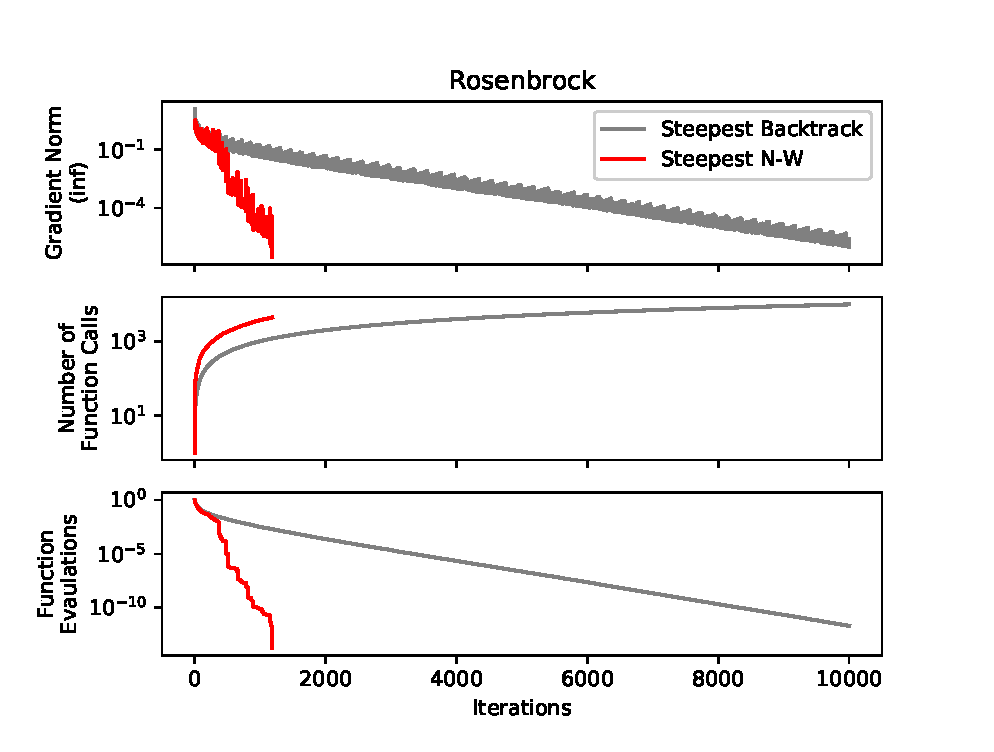
\includegraphics[width=0.45\textwidth]{figures/steepest_rosen.eps}
		\label{fig:sub1}
	}
	\qquad
	\subfloat[]{
		\includegraphics[width=0.45\textwidth]{figures/quasi_rosen.eps}
		\label{fig:sub2}
	}
	\caption{The comparisons of the gradient norm, number of function calls, and the function evaluations verses the number of iterations for the Rosenbrock test case at the starting point of [-2,2]. Notice how the algorithm converges to zeros using the N-W method a lot faster than the backtrack method.}
	\label{fig:rosen}
\end{figure}

\begin{figure}[htbp]
	\centering
	\subfloat[]{
		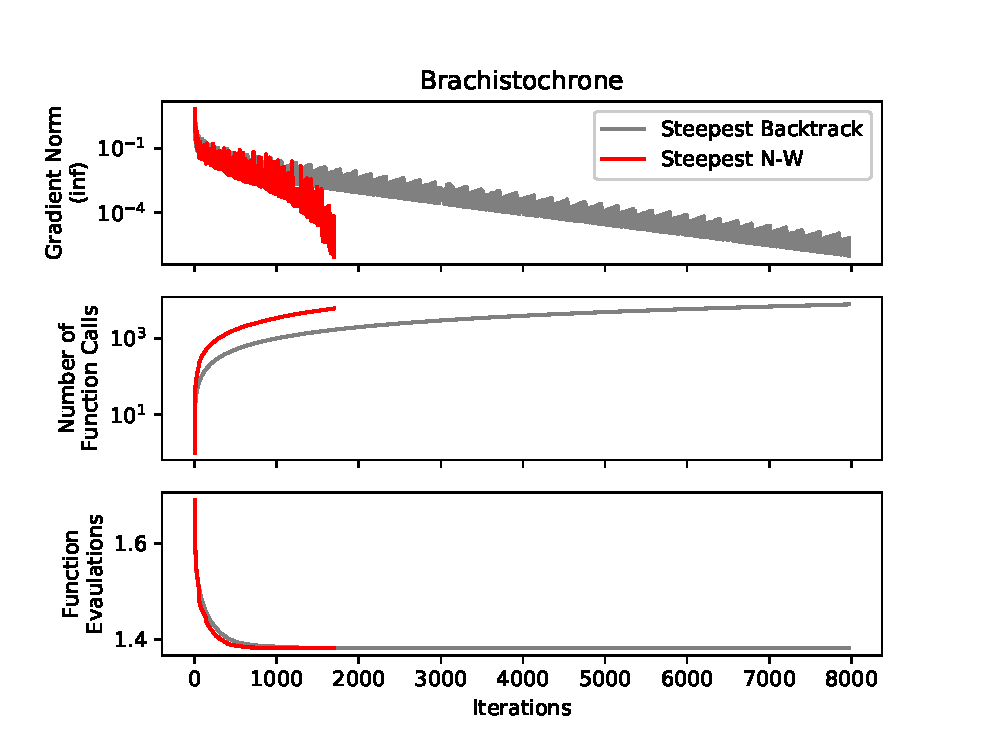
\includegraphics[width=0.45\textwidth]{figures/steepest_brach.eps}
		\label{fig:sub1}
	}
	\qquad
	\subfloat[]{
		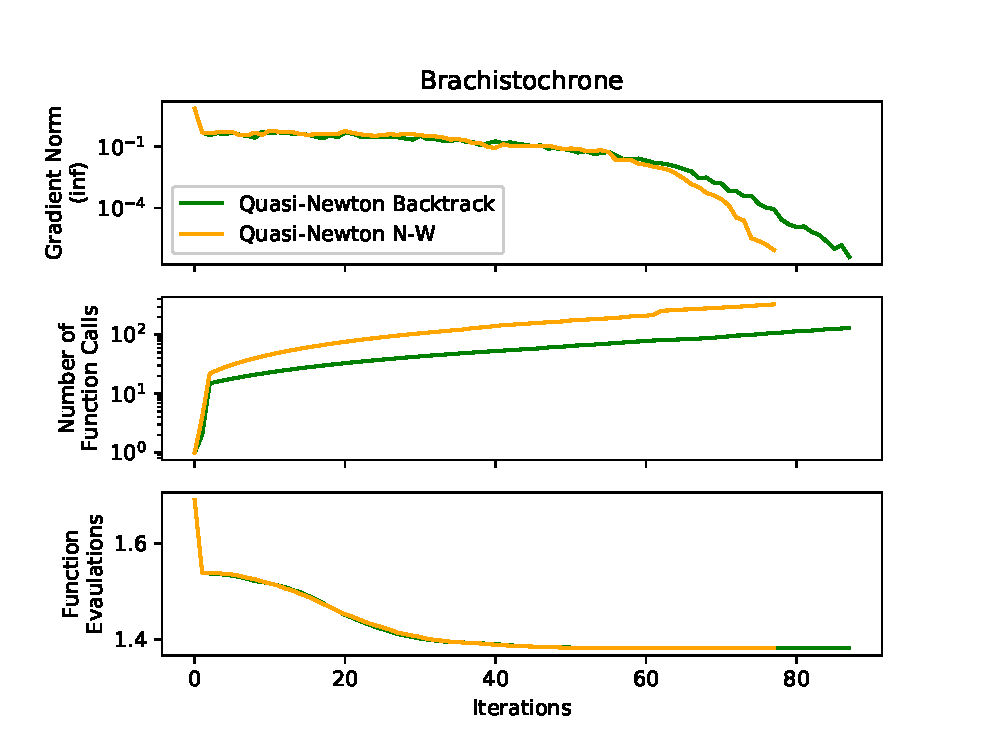
\includegraphics[width=0.45\textwidth]{figures/quasi_brach.eps}
		\label{fig:sub2}
	}
	\caption{The comparisons of the gradient norm, number of function calls, and the function evaluations verses the number of iterations for the Brachistrochrone test case using 60 points. In this case the Quasi-Newton Backtrack levels out at fewer number of function calls than Quasi-Newton N-W but has more iterations. }
	\label{fig:brach}
\end{figure}



We also chose to compare these algorithms to the python library \href{https://docs.scipy.org/doc/scipy/reference/generated/scipy.optimize.minimize.html}{scipy}, using the same starting points which were selected randomly. The starting points are shown in \Cref{tab:start_pts} and the corresponding average number of function calls is shown in Table 5. Overall, the python library does the best. 


\begin{table}
	\parbox{.3\linewidth}{
		\centering
		\caption{Uniform random starting points to test convergence.}
		\label{tab:start_pts}
		\begin{tabular}{c|c}
			\toprule
			X1 & x2 \\
			\midrule
			-62.30386999 & -25.83768453 \\
			-21.0403251 & -14.02330778 \\
			9.70891713 & -67.46296481 \\
			-96.17539178 & -80.59439791 \\
			-1.84957355 & 25.32791886 \\
			63.62334595 & 76.05005117 \\
			-15.88931528 & -85.03483885 \\
			19.42054044 & 67.07047287 \\
			47.82754075 & -57.23680417 \\
			85.25710413 & 26.2181083 \\
			\bottomrule
		\end{tabular}
	}
	\hfill
	\parbox{.65\linewidth}{
		\centering
		\label{tab:average_func_calls}
		\caption{The results of starting the Maytas and the Rosenbrock functions at different starting locations \Cref{tab:start_pts} and comparing the average number of function calls to scipy minimize function. For the Brachistochrone function, it doesn't make sense to have random starting points and so we tested only 256 points linearly initialized between the endpoints.}
		\begin{tabular}{c|c}
			\toprule
			Algorithm & Average Function Calls \\
			\midrule
			Matyas Scipy & 13.5 \\
			Matyas Quasi-Newton N-W & 93.1 \\
			Rosenbrack Scipy & 267.5 \\
			Rosenbrack Quasi-Newton N-W & 4907.3 \\
			Brachistochrone Scipy & 467 \\
			Brachistochrone Quasi-Newton N-W & 2015 \\
			\bottomrule
		\end{tabular}
	}
\end{table}



\section*{Conclusions}

Overall it was challenging to make these algorithms robust. The Matyas and Rosenbrock worked well for test cases close to their solutions but as I started to try other starting points far away, the algorithms had trouble. Even steepest descent seemed to make no progress. I finally choose the Quasi-Newton N-W method because it consistently solved the problems. 

If I were to improve anything about my implementations it would be to make sure that I am not calling the function when I don't need to be. There seemed to be some points in the bracketing and pinpointing algorithm that I could do this. I would also make the algorithm more robust to vanishing or exploding gradients. This seemed to be my biggest issues because they cause my step sizes to take either huge steps or hardly no step at all.

I learned a lot about implementing gradient based optimization. I can now use other optimization tools a little better because I learned about what is going on under the hood to a small extent. This assignment was a good experience and introduction in basic optimization techniques.
% This is for the bibliography.  Note that it is using sample.bib 
% you would need to provide your own bibtex file.

\bibliographystyle{unsrt}
\bibliography{sample}




\end{document}